% =========================
% sections/device_process.tex
% =========================
\section{Device and Process Integration}

\subsection{LPDDR Technology Background}
Low-power DRAM (LPDDR) is the de facto main memory for mobile systems, providing tens to a few hundreds of~GB/s bandwidth
at substantially lower I/O energy than HBM-class DRAM~\cite{ChoiIEDM2022}.
Despite architectural and I/O optimizations, LPDDR is \emph{volatile} and incurs standby power due to periodic refresh.

% --- Fig.2: 特性比較 ---
% figures/fig2_access_retention.tex
\begin{figure}[t]
  \centering
  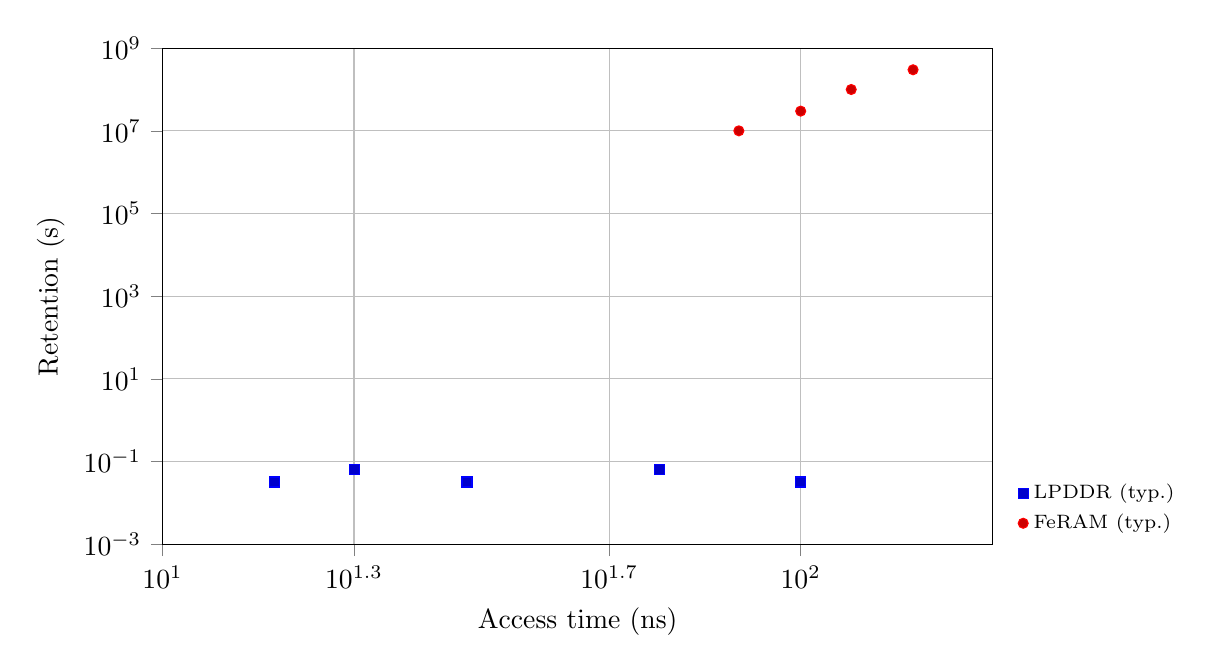
\begin{tikzpicture}
    \begin{loglogaxis}[
      width=\columnwidth,
      height=0.65\columnwidth,
      xlabel={Access time (ns)},
      ylabel={Retention (s)},
      legend style={at={(1.02,0)},anchor=south west, draw=none, fill=white, font=\scriptsize}, % ← 外側
      legend cell align=left,
      grid=both,
      tick align=outside,
      tickpos=left,
      xmin=10, xmax=200,
      ymin=1e-3, ymax=1e9,
      ytickten={-3,-1,1,3,5,7,9},
      xtickten={1,1.3,1.7,2},
      clip=false % ← 凡例が外に出る時の保険
    ]

    % LPDDR
    \addplot+[only marks, mark=square*, mark size=1.8pt]
    coordinates {(15,3.2e-2) (20,6.4e-2) (30,3.2e-2) (60,6.4e-2) (100,3.2e-2)};
    \addlegendentry{LPDDR (typ.)}

    % FeRAM
    \addplot+[only marks, mark=*, mark size=1.8pt]
    coordinates {(80,1.0e7) (100,3.0e7) (120,1.0e8) (150,3.0e8)};
    \addlegendentry{FeRAM (typ.)}

    \end{loglogaxis}
  \end{tikzpicture}
  \vspace{-0.6em}
  \caption{Access time vs.\ retention.}
  \label{fig:access_retention_lpddr_feram}
\end{figure}


\subsection{FeRAM Device and Process}
Ferroelectric RAM (FeRAM) based on doped HfO$_2$ leverages polarization switching to store data with low write voltage and fast access~\cite{MullerAPL2011,KimIEDM2021,NohedaNRM2023}.
Process-wise, FeRAM/FeFET flows require \emph{low-to-mid} temperature stabilization ($\sim$350--450$\,^\circ\mathrm{C}$) to preserve the ferroelectric orthorhombic phase in HfZrO$_2$.

\subsection{Why Monolithic Co-Integration Is Impractical}
LPDDR DRAM arrays rely on high-temperature anneals ($>700\,^\circ\mathrm{C}$) to realize high-quality storage capacitors.
Such thermal budgets collapse the ferroelectric phase of HfO$_2$, whereas post-FeRAM low-temperature windows cannot support DRAM capacitor quality.
Therefore, monolithic LPDDR+FeRAM co-fabrication is \textbf{impractical}; a package-level approach is required.

\subsection{Package-Level Integration: Chiplet/SiP/PoP}
Figure~\ref{fig:package_lpddr_feram} shows our organization:
(1) LPDDR remains as a standard DRAM die/package optimized in its own process;
(2) a small FeRAM die (chiplet) is co-packaged on a common substrate (SiP/interposer or PoP);
(3) the SoC connects to both through short, low-parasitic interconnects.
This separation preserves each technology's process window while enabling system-level policies to exploit non-volatility.

% --- Fig.3: パッケージ統合(ノード明記) ---
\begin{figure}[t]
\centering
\begin{tikzpicture}[
  node/.style={draw, rounded corners=2pt, align=center, inner sep=4pt},
  arrow/.style={-Latex}
]
\node[node, fill=gray!10] (soc) {SoC (CPU/GPU/NPU)\\\small 5--3\,nm FinFET/GAAFET};
\node[node, fill=green!10, right=1.8cm of soc] (lpddr) {LPDDR5/5X\\\small 1$\alpha$--1$\gamma$ (14--10\,nm)};
\node[node, fill=blue!10, below=1.2cm of lpddr] (feram) {FeRAM chiplet\\\small 28--22\,nm CMOS\\\small HfO$_2$ ferroelectric};
\node[node, fill=orange!10, below=1.2cm of soc, text width=2.9cm] (sysdk) {SystemDK / OS\\\small checkpoint/resume\\\small refresh offload};

\draw[arrow] (soc) -- (lpddr) node[midway, above] {\small high BW};
\draw[arrow] (lpddr) -- (soc);
\draw[arrow] (lpddr) -- (feram) node[midway, right] {\small ckpt};
\draw[arrow] (feram) -- (lpddr);
\draw[arrow] (sysdk) -- (lpddr);
\draw[arrow] (sysdk) -- (feram);
\end{tikzpicture}
\caption{Chiplet/SiP package-level integration with explicit process nodes.}
\label{fig:package_lpddr_feram}
\end{figure}

\subsection{Interface and Policy Hooks}
The FeRAM chiplet exposes a narrow, reliable link (e.g., mailbox DMA or AXI-lite) for:
\begin{itemize}
  \item \textbf{Checkpoint Write/Read}: bulk DMA of model/activation checkpoints and OS state.
  \item \textbf{Refresh Offloading}: firmware migrates cold regions from LPDDR to FeRAM, suppressing refresh traffic.
  \item \textbf{Instant Resume}: fast restore path avoiding full DRAM warm-up.
\end{itemize}
These hooks are orchestrated by the \emph{SystemDK} co-design framework (policies spanning architecture, package, and OS).

\subsection{Process Node Mapping}
To clarify manufacturability, Table~\ref{tab:node_mapping} summarizes representative nodes for each component.

\begin{table}[t]
  \centering
  \caption{Representative process nodes for LPDDR+FeRAM integration.}
  \label{tab:node_mapping}
  \vspace{2pt}
  \small
  \setlength{\tabcolsep}{5pt}
  \begin{tabular}{@{}lcll@{}}
    \toprule
    \textbf{Target} & \textbf{Node} & \textbf{Tech} & \textbf{Notes} \\
    \midrule
    SoC logic & 5--3\,nm & FinFET/GAAFET & Perf/W optimization \\
    LPDDR5/5X DRAM & 1$\alpha$--1$\gamma$ & 14--10\,nm DRAM & vendor “1x” gens \\
    FeRAM chiplet & 28--22\,nm & CMOS+ferroelectric & mature BEOL window \\
    Future FeFET & $<$10\,nm & CMOS-compatible & monolithic option \\
    \bottomrule
  \end{tabular}
\end{table}

\subsection{Key Technology Parameters}
Table~\ref{tab:tech_params} summarizes representative parameters used in our analysis (also reflected in Fig.~\ref{fig:access_retention_lpddr_feram}).
Values are order-of-magnitude estimates for policy exploration; silicon-specific tuning is straightforward.

\begin{table}[t]
  \centering
  \caption{Representative parameters for LPDDR and FeRAM used in evaluation.}
  \label{tab:tech_params}
  \vspace{2pt}
  \small
  \setlength{\tabcolsep}{5pt}
  \begin{tabular}{@{}lcc@{}}
    \toprule
    Parameter & LPDDR (typical) & FeRAM (typical) \\
    \midrule
    Access latency & 15--60~ns & 80--150~ns \\
    Retention & volatile (32--64~ms refresh) & $10^7$--$10^8$~s ($\sim$years) \\
    Write energy/bit & moderate & low \\
    Endurance & $>10^{15}$ accesses & $10^8$--$10^{12}$ writes \\
    Process temperature & capacitor anneal $>700\,^\circ$C & 350--450$\,^\circ$C \\
    Role & working memory & checkpoint/state \\
    \bottomrule
  \end{tabular}
\end{table}

\subsection{Comparison with Other NVM Options}
Beyond FeRAM, several emerging NVMs are considered for assistive integration.
Table~\ref{tab:nvm_comparison} summarizes key features of ReRAM, MRAM, and FeFET relative to FeRAM.
This comparison motivates our choice of FeRAM chiplets for near-term manufacturability, while clarifying future upgrade paths.

\begin{table}[t]
  \centering
  \caption{Comparison of candidate NVM options for LPDDR assistive integration.}
  \label{tab:nvm_comparison}
  \vspace{2pt}
  \small
  \setlength{\tabcolsep}{4pt}
  \begin{tabular}{@{}lcccc@{}}
    \toprule
    & FeRAM & ReRAM & MRAM & FeFET \\
    \midrule
    Write speed & 10~ns & 50--100~ns & 1--10~ns & 1--10~ns \\
    Retention   & $10^7$--$10^8$~s & $10^5$--$10^6$~s & $>10$~years & $10^6$--$10^7$~s \\
    Endurance   & $10^8$--$10^{12}$ & $10^6$--$10^9$ & $>10^{15}$ & $10^6$--$10^9$ \\
    Process temp. & 350--450$^\circ$C & BEOL-friendly & BEOL mismatch & $<$400$^\circ$C \\
    Integration  & CMOS-compatible & CMOS-friendly & MTJ-specific & Gate-stack CMOS \\
    Maturity     & High & Medium & High & Emerging \\
    \bottomrule
  \end{tabular}
\end{table}
